\documentclass[]{article}
\usepackage{lmodern}
\usepackage{amssymb,amsmath}
\usepackage{ifxetex,ifluatex}
\usepackage{fixltx2e} % provides \textsubscript
\ifnum 0\ifxetex 1\fi\ifluatex 1\fi=0 % if pdftex
  \usepackage[T1]{fontenc}
  \usepackage[utf8]{inputenc}
\else % if luatex or xelatex
  \ifxetex
    \usepackage{mathspec}
  \else
    \usepackage{fontspec}
  \fi
  \defaultfontfeatures{Ligatures=TeX,Scale=MatchLowercase}
\fi
% use upquote if available, for straight quotes in verbatim environments
\IfFileExists{upquote.sty}{\usepackage{upquote}}{}
% use microtype if available
\IfFileExists{microtype.sty}{%
\usepackage{microtype}
\UseMicrotypeSet[protrusion]{basicmath} % disable protrusion for tt fonts
}{}
\usepackage[margin=1in]{geometry}
\usepackage{hyperref}
\hypersetup{unicode=true,
            pdftitle={Import data to RStudio},
            pdfauthor={Jeff Wesner},
            pdfborder={0 0 0},
            breaklinks=true}
\urlstyle{same}  % don't use monospace font for urls
\usepackage{graphicx,grffile}
\makeatletter
\def\maxwidth{\ifdim\Gin@nat@width>\linewidth\linewidth\else\Gin@nat@width\fi}
\def\maxheight{\ifdim\Gin@nat@height>\textheight\textheight\else\Gin@nat@height\fi}
\makeatother
% Scale images if necessary, so that they will not overflow the page
% margins by default, and it is still possible to overwrite the defaults
% using explicit options in \includegraphics[width, height, ...]{}
\setkeys{Gin}{width=\maxwidth,height=\maxheight,keepaspectratio}
\IfFileExists{parskip.sty}{%
\usepackage{parskip}
}{% else
\setlength{\parindent}{0pt}
\setlength{\parskip}{6pt plus 2pt minus 1pt}
}
\setlength{\emergencystretch}{3em}  % prevent overfull lines
\providecommand{\tightlist}{%
  \setlength{\itemsep}{0pt}\setlength{\parskip}{0pt}}
\setcounter{secnumdepth}{0}
% Redefines (sub)paragraphs to behave more like sections
\ifx\paragraph\undefined\else
\let\oldparagraph\paragraph
\renewcommand{\paragraph}[1]{\oldparagraph{#1}\mbox{}}
\fi
\ifx\subparagraph\undefined\else
\let\oldsubparagraph\subparagraph
\renewcommand{\subparagraph}[1]{\oldsubparagraph{#1}\mbox{}}
\fi

%%% Use protect on footnotes to avoid problems with footnotes in titles
\let\rmarkdownfootnote\footnote%
\def\footnote{\protect\rmarkdownfootnote}

%%% Change title format to be more compact
\usepackage{titling}

% Create subtitle command for use in maketitle
\providecommand{\subtitle}[1]{
  \posttitle{
    \begin{center}\large#1\end{center}
    }
}

\setlength{\droptitle}{-2em}

  \title{Import data to RStudio}
    \pretitle{\vspace{\droptitle}\centering\huge}
  \posttitle{\par}
    \author{Jeff Wesner}
    \preauthor{\centering\large\emph}
  \postauthor{\par}
      \predate{\centering\large\emph}
  \postdate{\par}
    \date{September 19, 2019}


\begin{document}
\maketitle

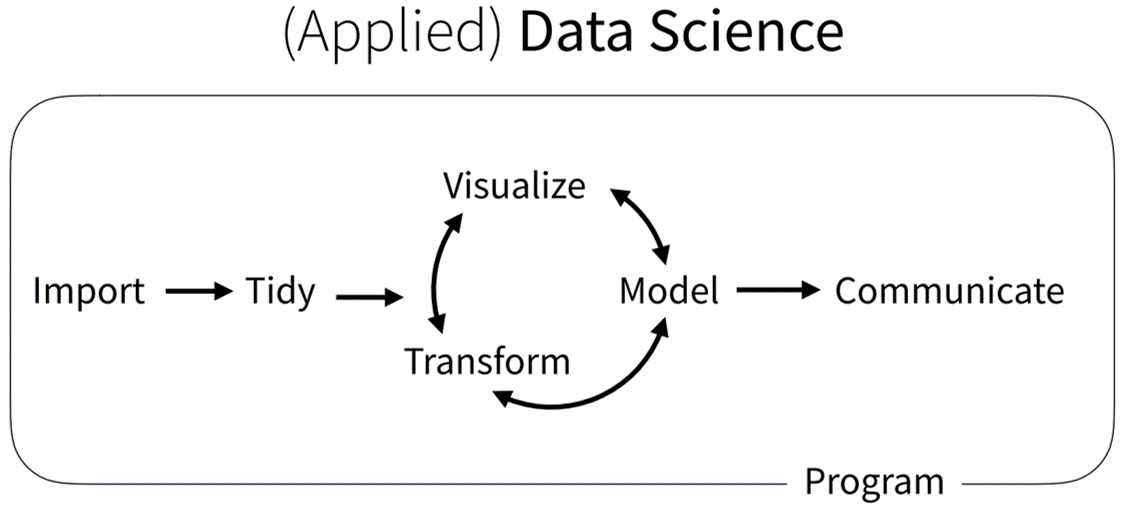
\includegraphics{data_workflow.png} Nearly every study that includes
data has a workflow similar to that above. We gather data, get it into a
program (Import), get it in the right format (Tidy), and then analyze it
with plots (Visualiation), Models, Transformations, etc. When we've
finished, we communicate the results to our peers. You'll learn how to
complete these steps in R because its designed specifically for each of
these steps. But the workflow applies regardless of the software you
use.

\subsection{1) Get data from Gapminder}\label{get-data-from-gapminder}

For this example, we'll work with a dataset of fertility rates. Go to
\url{https://www.gapminder.org/data/}. Search for ``children per woman
total fertility''. Download the csv and save it to a folder on your
computer that you will remember.

\subsection{2) Create a project}\label{create-a-project}

Open RStudio and create a project in the same folder as your dataset:

\emph{File -\textgreater{} New Project\ldots{} -\textgreater{} Existing
Directory -\textgreater{} Browse -\textgreater{}} {[}NAME OF YOUR
FOLDER{]}

You only have to do this once. Everything you compute will be saved in
this project, and you can always start where you left off.

\subsection{3) Import the data to
RStudio}\label{import-the-data-to-rstudio}

Look in the lower right panel of RStudio. Click on ``Files''. Do you see
the Gapminder data you saved? Left-click on your dataset and choose
\emph{Import Dataset} like this:

\begin{figure}
\centering
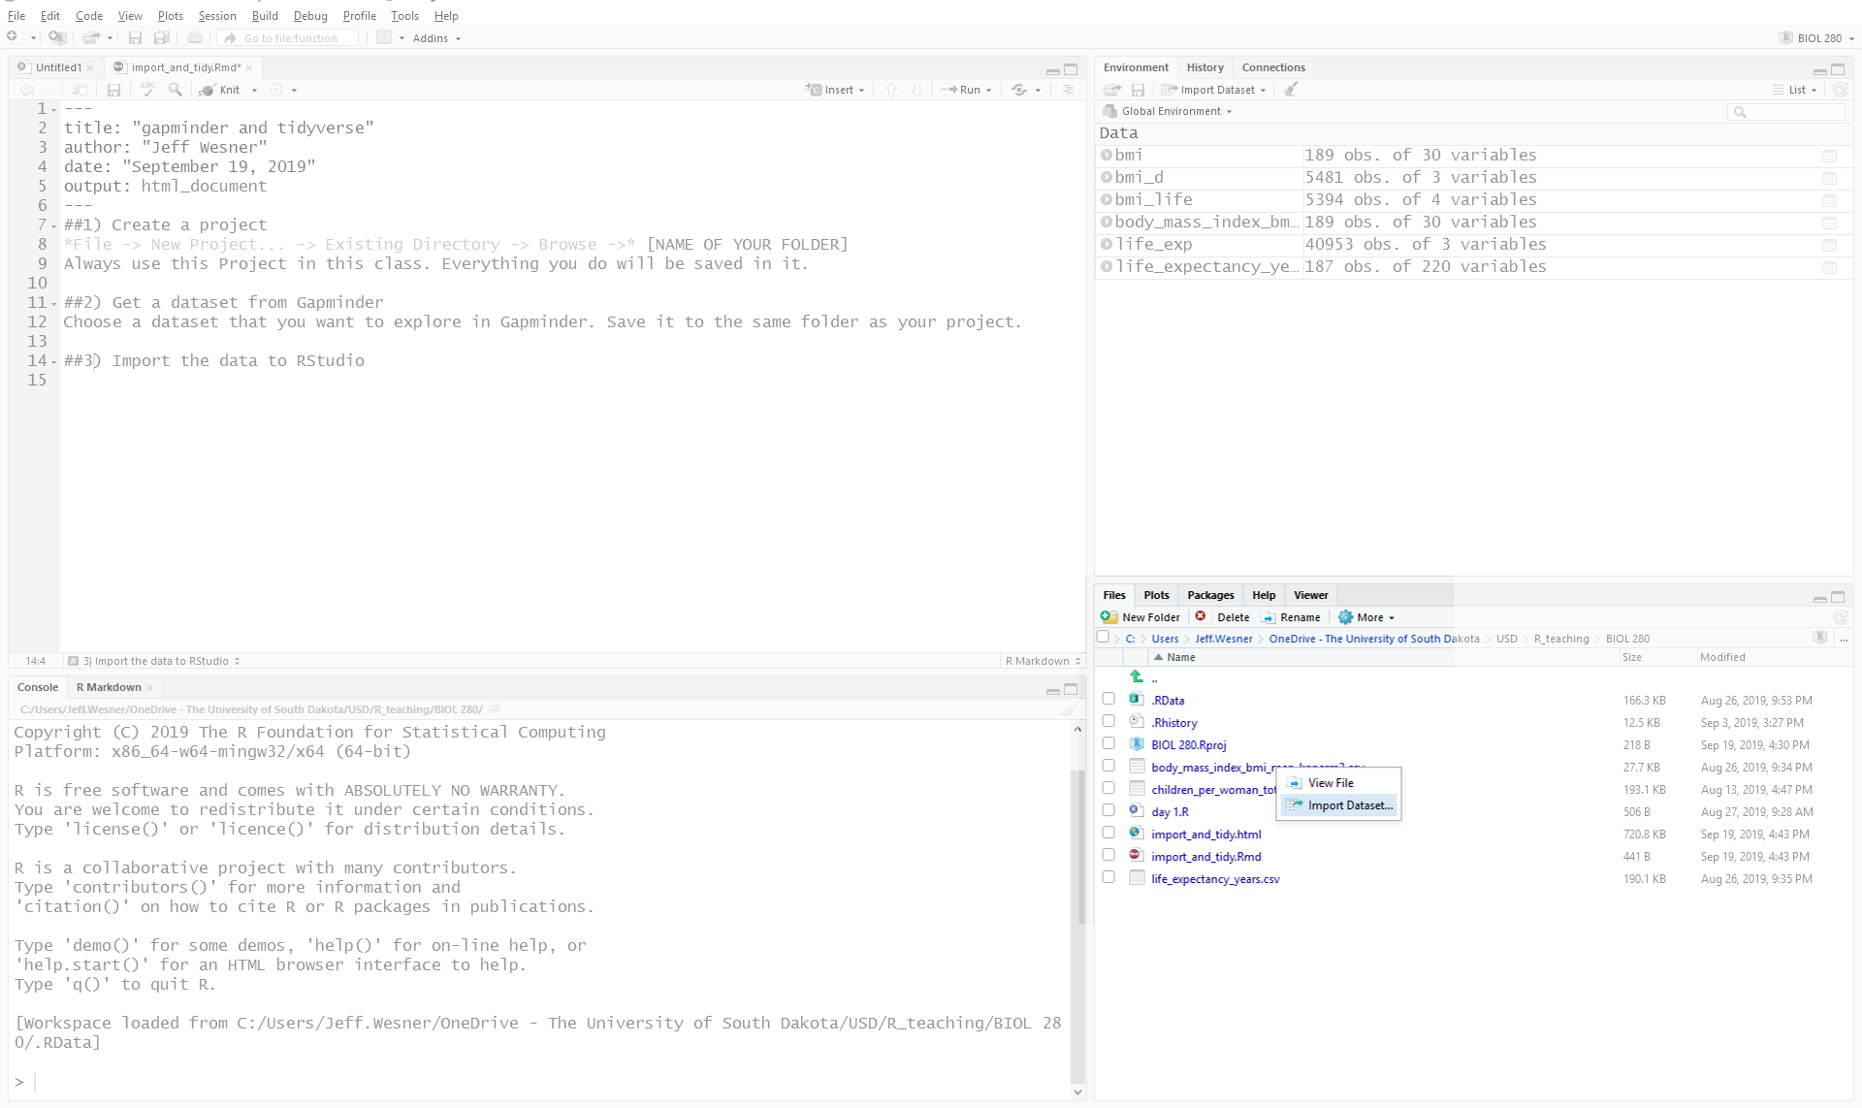
\includegraphics{import_example.png}
\caption{}
\end{figure}

After you click \emph{Import Dataset}, you'll see a preview of your
dataset like this:

\begin{figure}
\centering
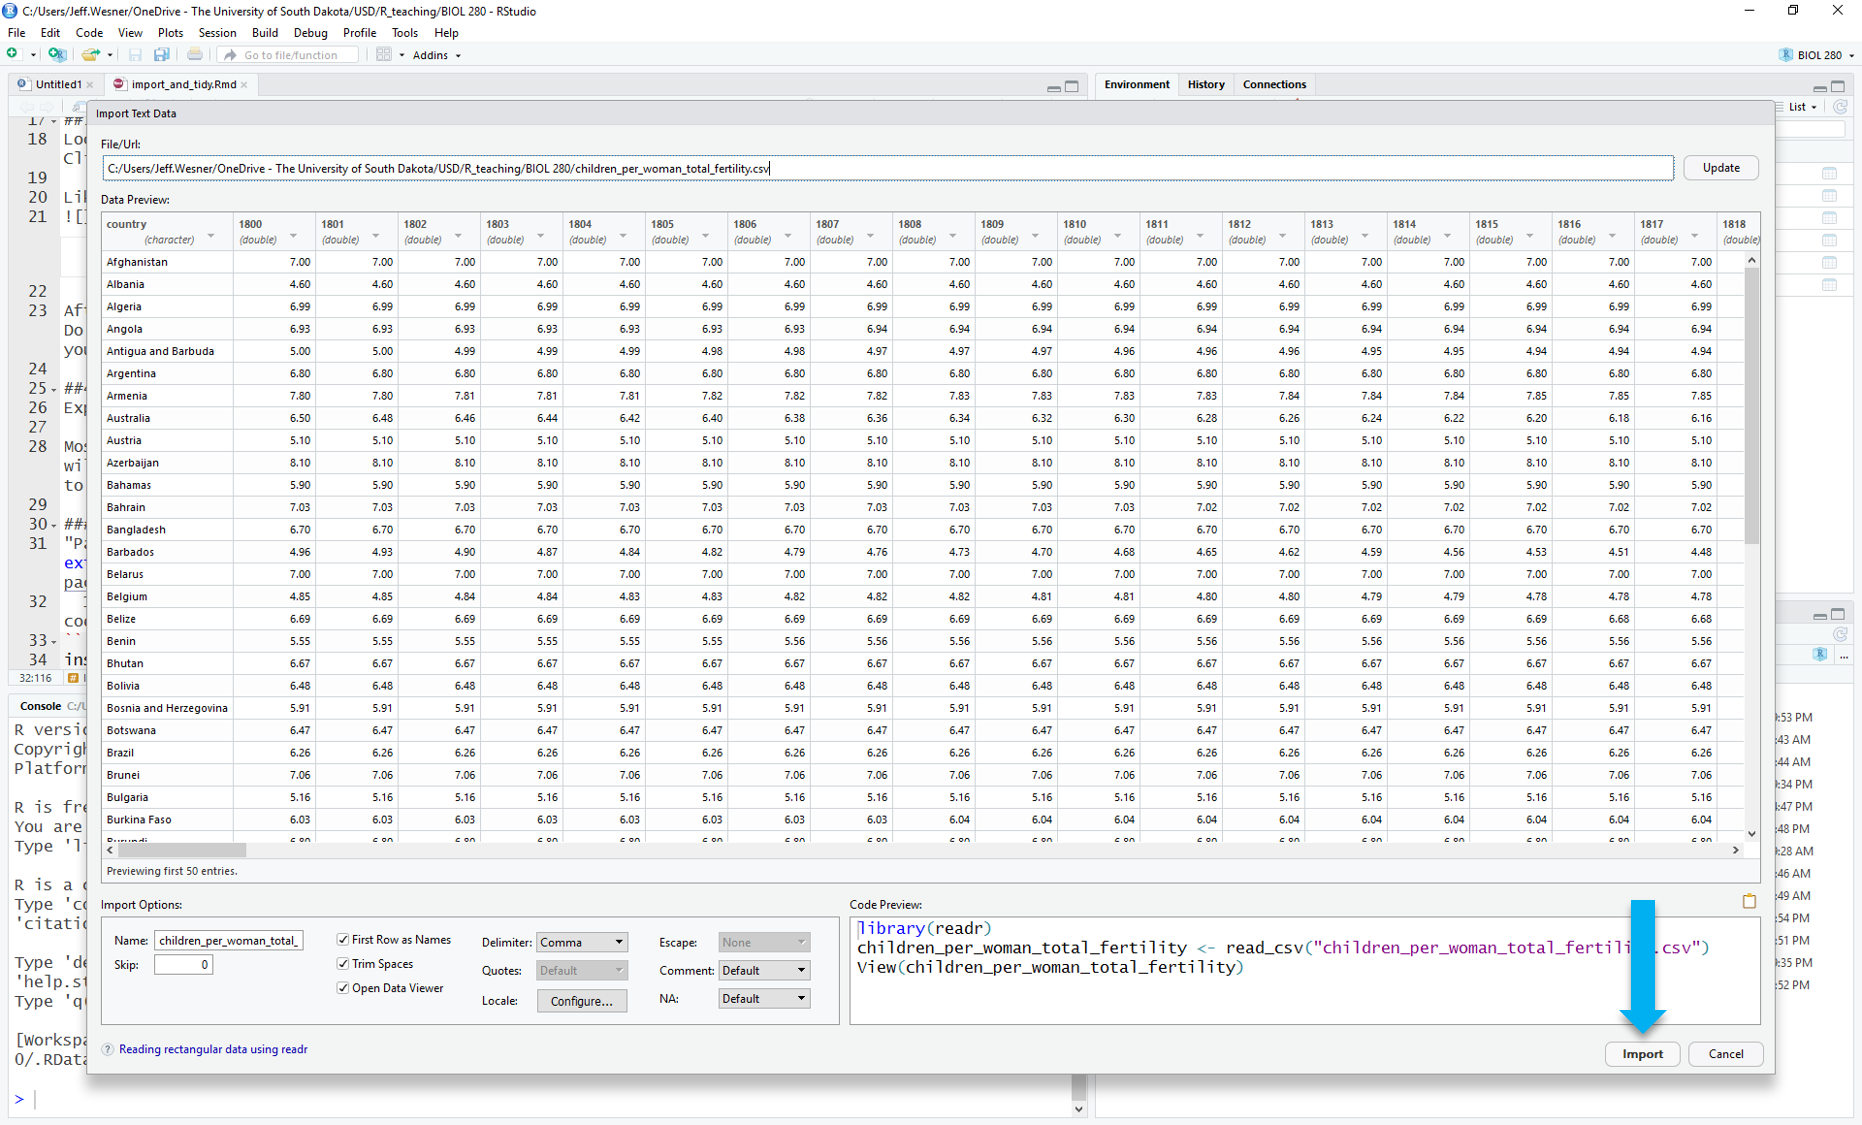
\includegraphics{import_button.png}
\caption{}
\end{figure}

Click \emph{Import} in the lower right.

Do you see the name of the dataset in the upper right panel? If so,
success! If not, re-try the steps above or ask your instructor.

Now explore your data. How many columns does it have? How many rows?
What are the variables?

Can you import a different dataset?


\end{document}
